\section{Evaluation}
\label{eval}
\noindent
We have discussed a potential loophole in android's custom provider data flow, in this paper. We are going to demonstrate four possible scenarios for this loophole through our experiments. In each case the vulnerability either already exists in the app or it was introduced by us. In scenario 1 we have an app that has the vulnerability and does nothing to protect itself and we know the exact uri call to access the content provider. Scenario 2 is where the app uses certificate key signatures to detect the reverse engineering and blocks any attempt to start the app itself. Scenario 3 is where the app does not crash at all and works like a normal app. However, when one tries to access a component of the app like a content provider the app includes custom access control checks. Scenario 4 is still under investigation, but this is the case  where an app's uri string can be fully obtained by a combination of parsing the Manifest file and guess work. In order to demonstrate this problem we built a proof-of-concept(PoC). All our experiments were ran on a LG Nexus 5 device with Android Marshmallow 6.0 installed on it.

\subsection{Scenario 1: Vulnerability with complete knowledge}
In our PoC, we have an app(COMMAND) that has an exported content provider. We created another app(Parser) that is capable of accessing the content provider. We use two different application package sets and observe the results. The first set contains the COMMAND app without any permission specification and Parser app without any permission request. The second set contains the COMMAND app with permission specification and association with the provider that was created. It also includes the Parser app with the request for the permission that was created by COMMAND. 

\subsubsection{PoC case 1 for permission control} COMMAND has associated permission, Parser has requested said permission. We see in Figure~\ref{fig:bothHavePerm} that, in this case there are no errors and we are able to make a sample query to the content provider.
\subsubsection{PoC case 2 for permission control} COMMAND has no associated permission, Parser has not requested said permission. We see in Figure~\ref{fig:neitherHavePerm} that, in this case there are no errors and we are again able to make a sample query to the content provider. We propose that there should a check in such a case to ensure that data access is to be allowed or denied. At present this does not happen and app developers resort to individual techniques to protect their data.
\begin{figure}
\centering
\begin{minipage}{.45\columnwidth}
	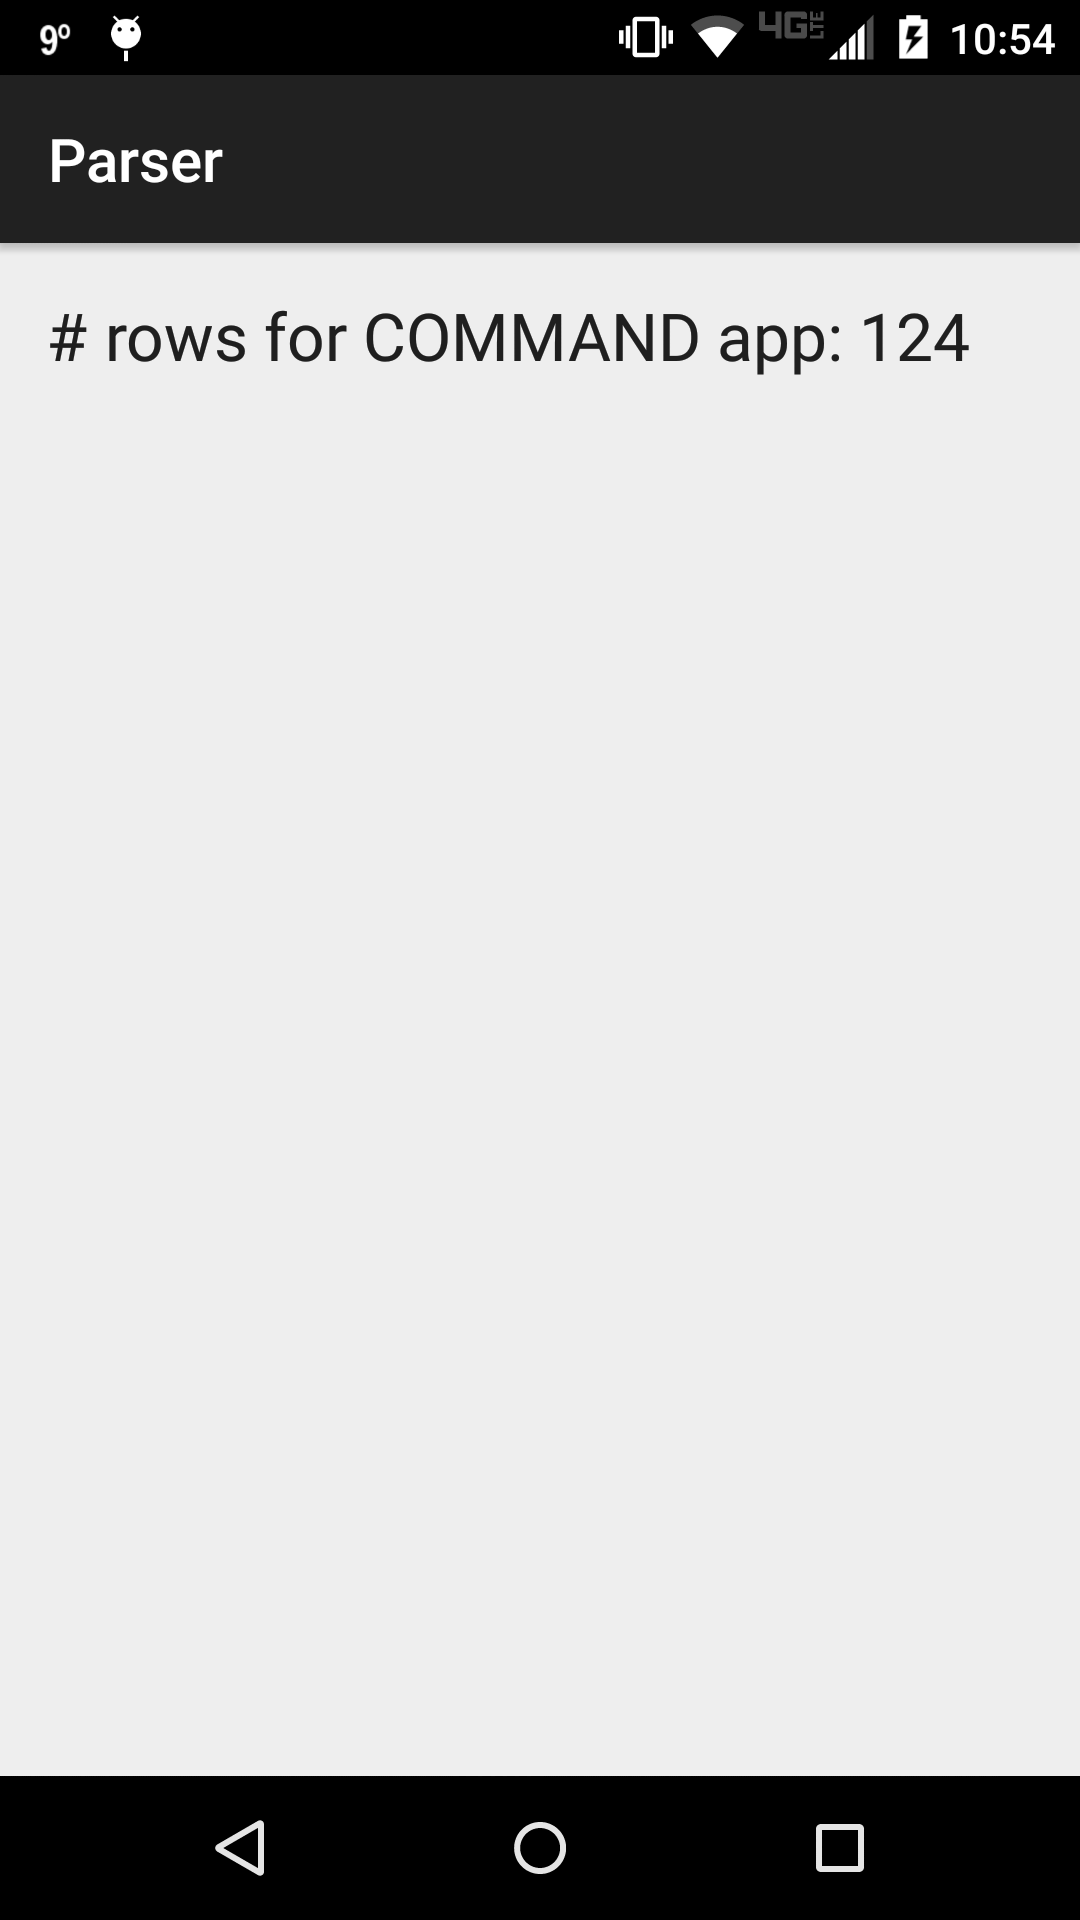
\includegraphics[width=\columnwidth,scale=0.5]{images/bothHavePerm}
	\caption{Android content provider accessed with permission}
	\label{fig:bothHavePerm}
\end{minipage}
\hspace{.05\linewidth}
\begin{minipage}{.45\columnwidth}
	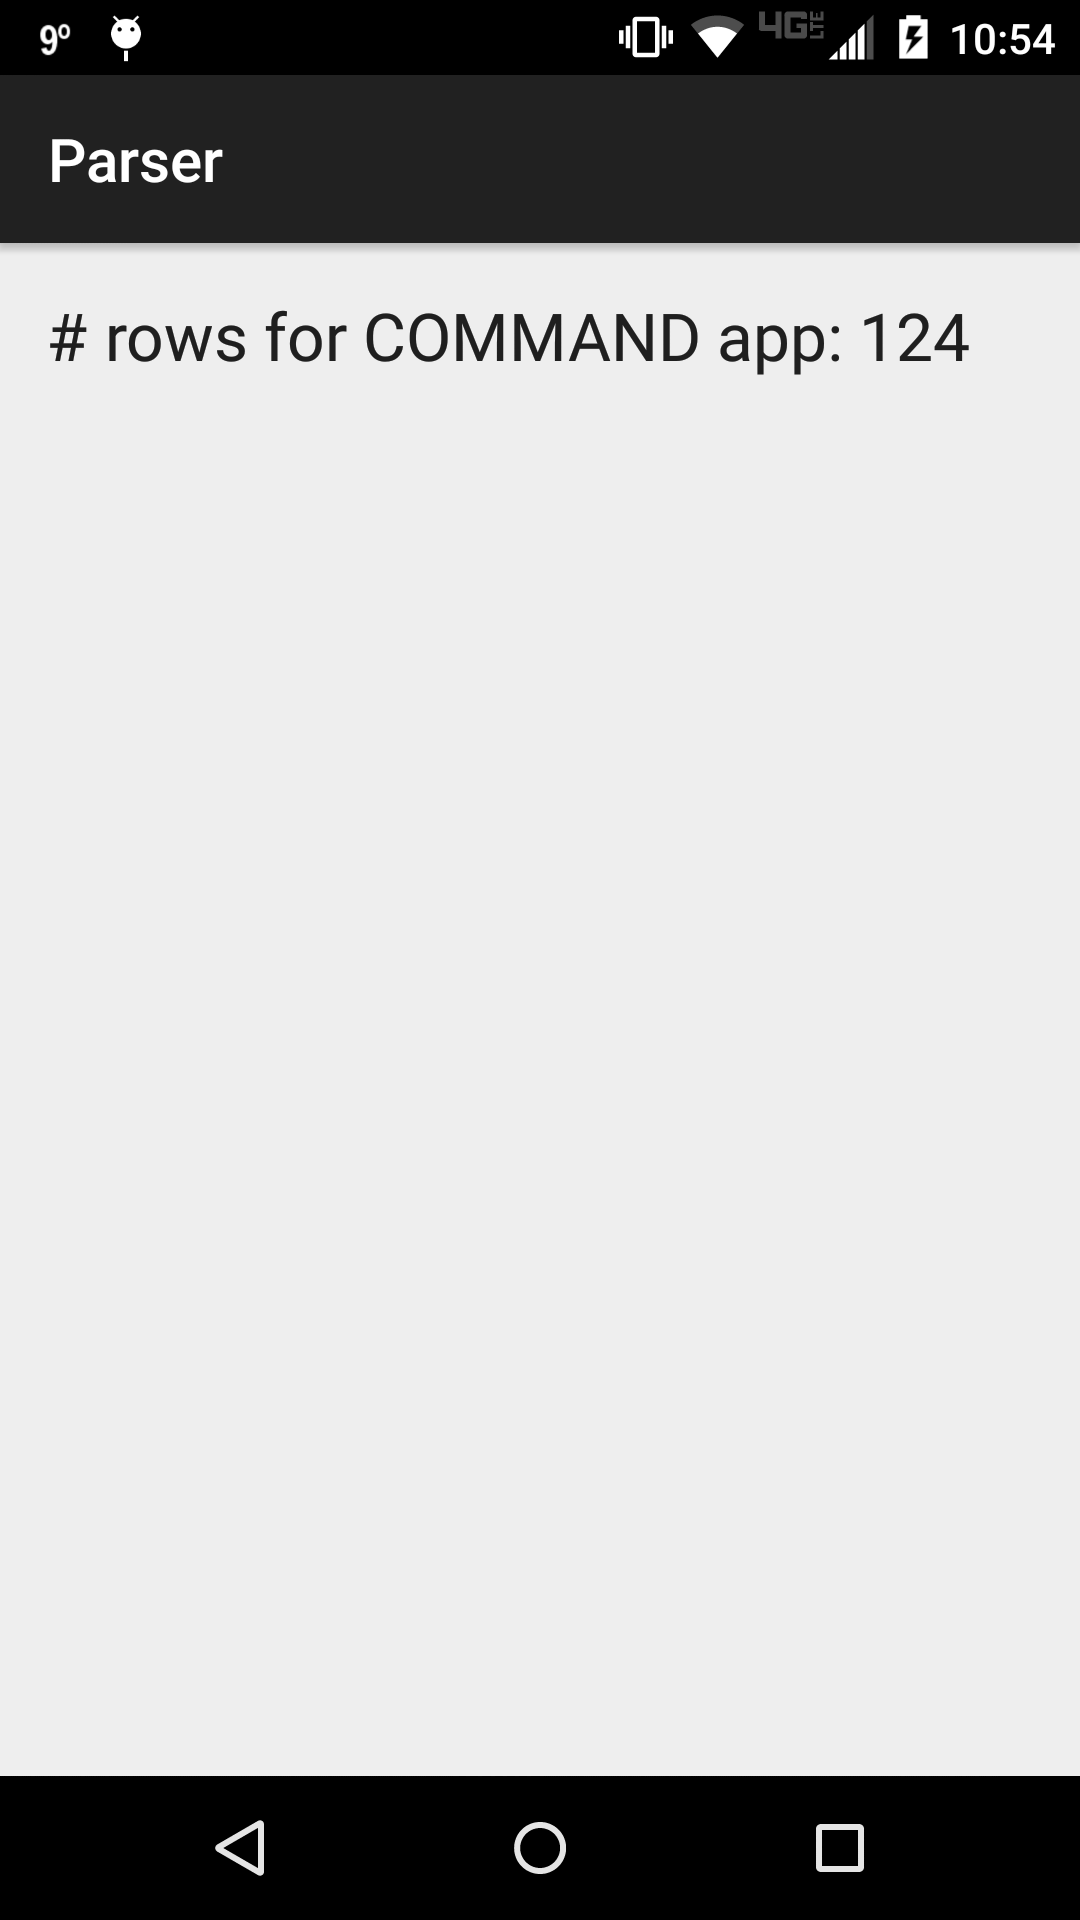
\includegraphics[width=\columnwidth,scale=0.5]{images/neitherHavePerm}
	\caption{Android content provider accessed without permission}
	\label{fig:neitherHavePerm}
\end{minipage}
\end{figure}
\subsubsection{PoC case 3 for permission control} COMMAND has associated permission, Parser has not requested said permission. We see in Figure~\ref{fig:didNotRequestPermission} that, causes a permission denial error which is what we expected.
\begin{figure}[tb]
\centering
	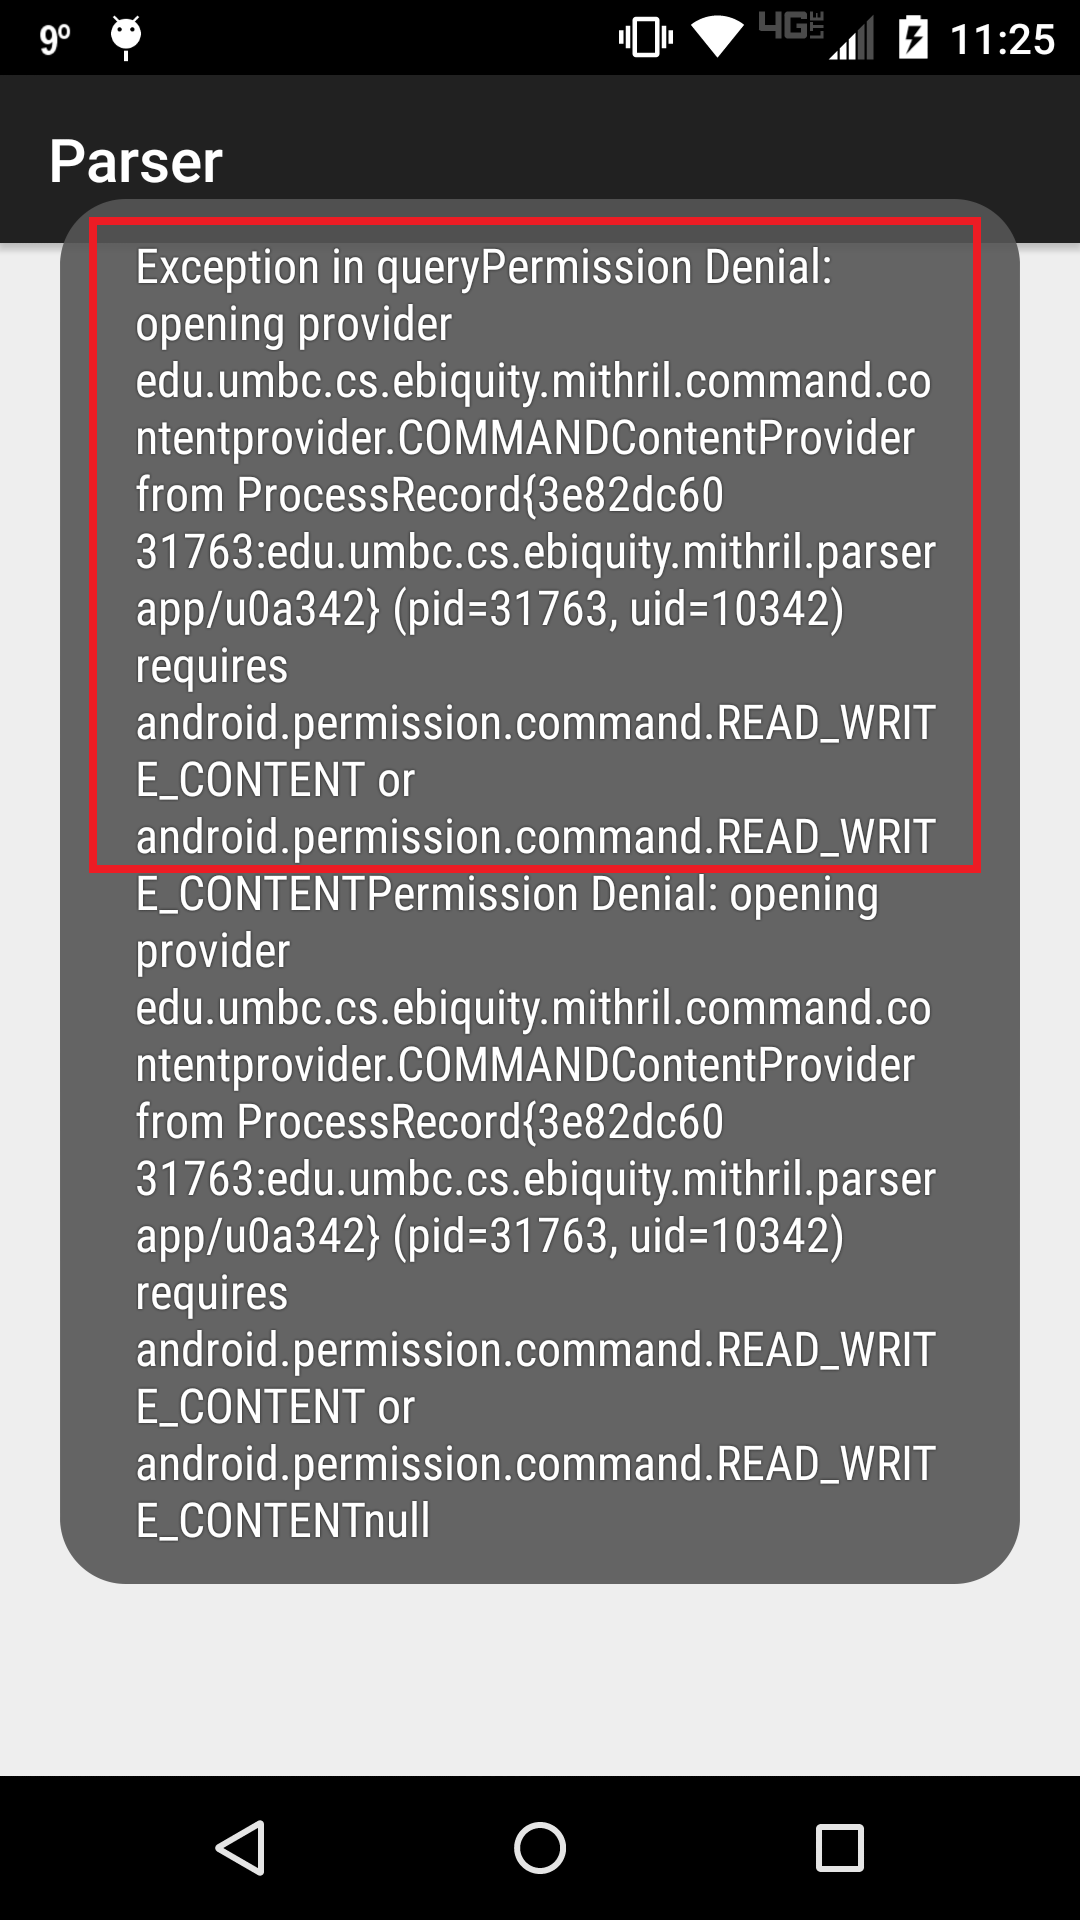
\includegraphics[scale=0.18]{images/didNotRequestPermission}
	\caption{Android content provider permission denial}
	\label{fig:didNotRequestPermission}
\end{figure}
\subsubsection{PoC case 4 for permission control} COMMAND has no associated permission, Parser has requested an unknown permission. There is no error in this case on the phone. We can ignore this error because this does not cause any leakage from the data provider perspective. The PoC proves that there is no difference from user perspective between an app which has a content provider with proper protection using appropriate permission and an app which does not have such access control implemented.

Therefore, user data can potentially leak without user knowledge. We ran our analysis on a set of 1500 randomly selected applications with a mix of popular applications like Facebook, GMail, Instagram as well as less popular and unknown apps like Expense Manager, Call App etc. Our system found 150 applications with provider set as exported and no associated permission for the provider. Therefore about 10\% of apps have this potential loophole but we wanted to find out if we could change an app to leak it's data. 

This led to our second set of experiments in trying to determine if these had incorporated additional protection apart from the standard android permission mechanisms. For these experiments we used the Facebook app and the Google Fit app. We removed all permissions associated with the providers on both the apps. We also set all the providers' exported setting to true.

\subsection{Scenario 2: App checks for signatures} Upon installation the Google fit app immediately crashed and kept on crashing every time we tried to use it. Therefore, in order to figure out the issue we used logcat, the Android logging system that provides a mechanism for collecting and viewing system debug output. We discovered from logcat messages that the Google Fit app had included an additional check on the app key signature and it simply crashed because the signature is detected as unknown. You can see the error in Figure~\ref{fig:GoogleProtections}.

\begin{figure}[tb]
\centering
	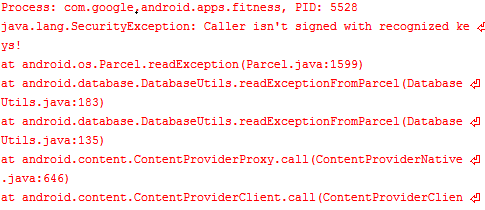
\includegraphics[width=\columnwidth]{images/GoogleProtections}
	\caption{Google Fit app checks for certificate signatures}
	\label{fig:GoogleProtections}
\end{figure}

\begin{figure}[tb]
\centering
	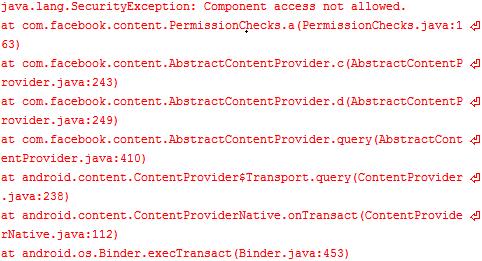
\includegraphics[width=\columnwidth]{images/FBProtections}
	\caption{Facebook checks controls access to it's component}
	\label{fig:FBProtections}
\end{figure}

\subsection{Scenario 3: App manages access control to it's components} For this case we used the Facebook app. We observed that the Facebook app never crashed and worked like a normal Facebook app. However, when we tried to access the app's content provider it blocked our attempts and you can see in Figure~\ref{fig:FBProtections} that it controls access to it's own component. Therefore, app developers are clearly detecting such issues on their apps but not always.

\begin{figure}[tb]
\centering
	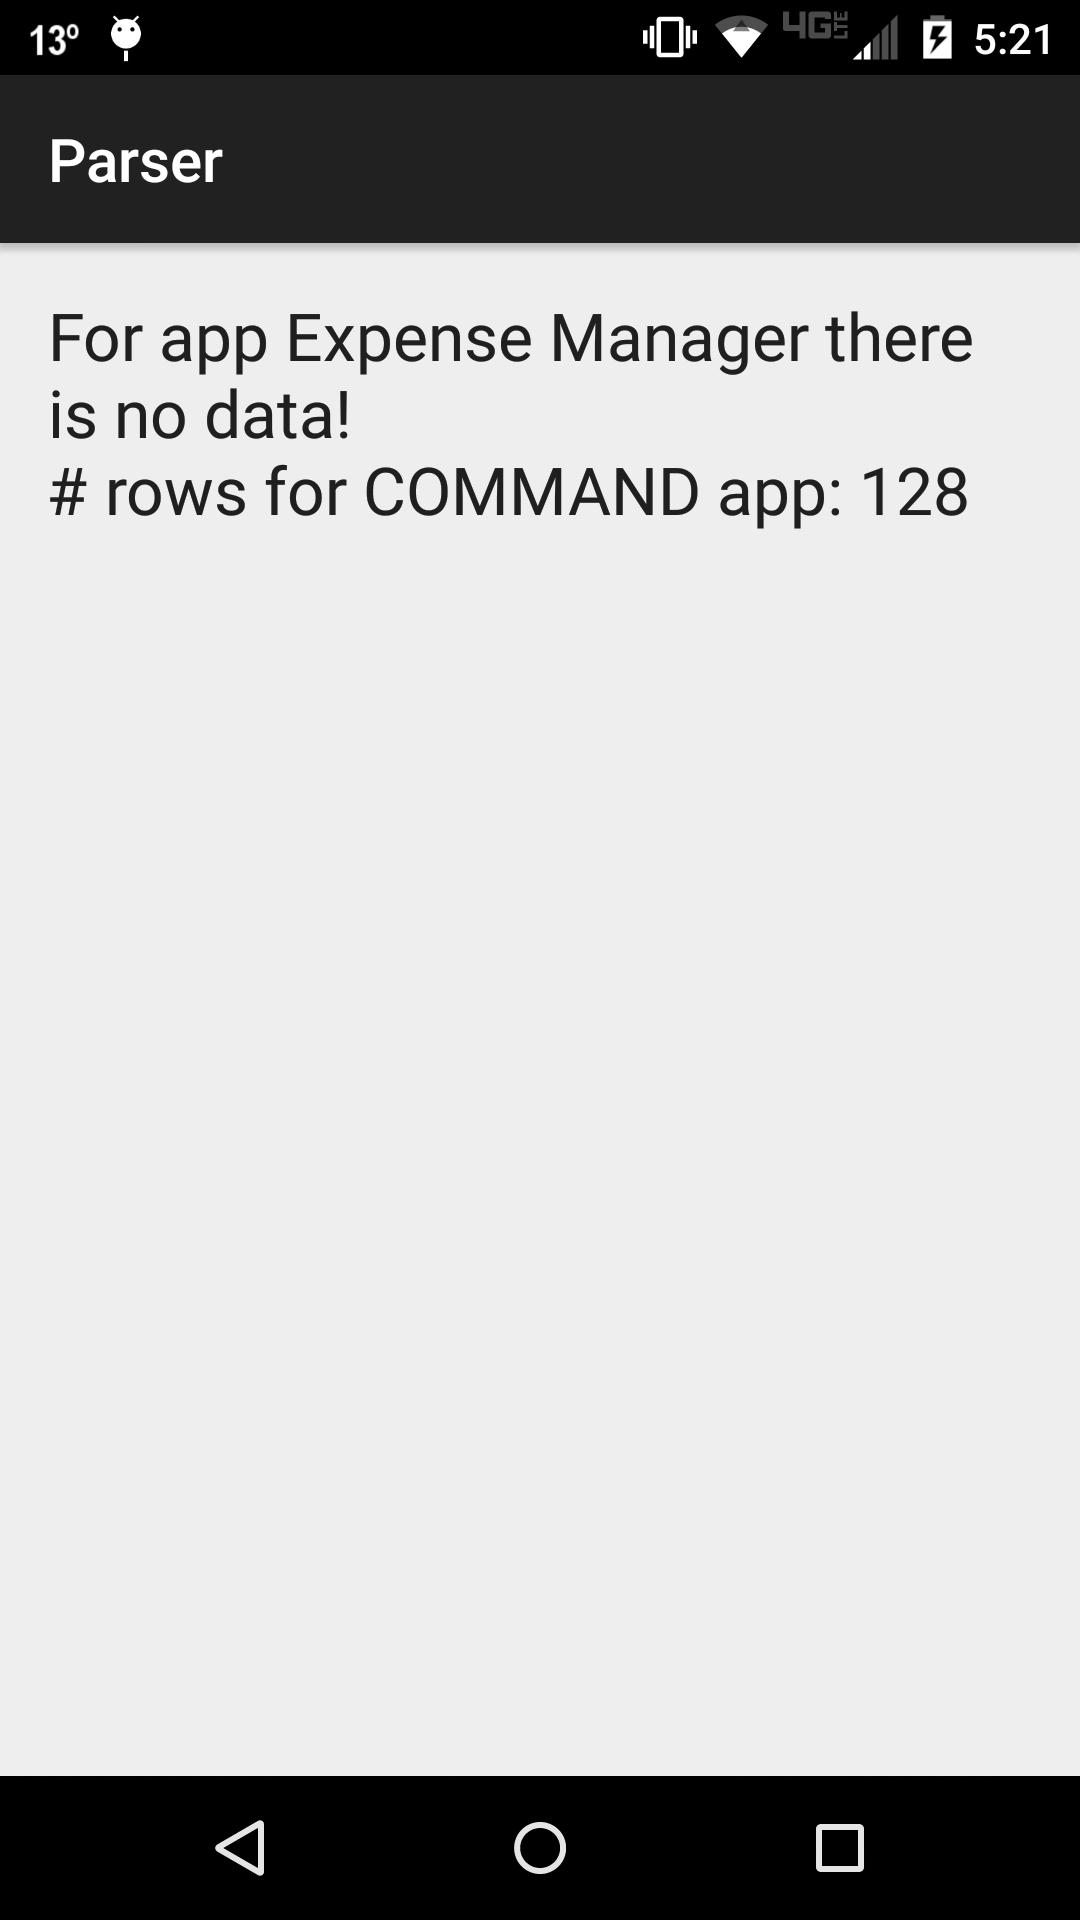
\includegraphics[scale=0.12]{images/nochecks}
	\caption{No check points were found on a less popular app}
	\label{fig:nochecks}
\end{figure}

\subsection{Scenario 4: Potentially vulnerable app} We found at least one app called Expense Management from our random sample set that allowed us access to it's content provider. However, we did not know the complete uri for the app's content provider. Therefore we had to make guesses. This app had not implemented any checkpoints or caused any errors as we saw in the other scenarios. You can see in Figure~\ref{fig:nochecks}, that our query did not return any data but that was because the app wasn't writing it's data to it's database. We are still investigating other apps for a potential breach that could lead to a full fledged exploit. We are currently processing more apps to find out if they include such checks as encoded by popular apps from Google or Facebook. This processing takes a long time as because we have to manually find the databases on the phone using a rooted phone and a SQLite explorer app. Thereafter, we have to make guesses for patterns that apps might have used in their content provider code. There are commonly used patterns like `\#' that can be used as a part of the URI to call the content provider in order to get access to the data and we are trying to use them to find out apps which have such a vulnerability.